
\documentclass[journal,12pt,twocolumn]{IEEEtran}
\usepackage{graphicx}
\usepackage[margin=0.5in]{geometry}
\graphicspath{{./figs/}}{}
\usepackage{amsmath,amssymb,amsfonts,amsthm}
\newcommand{\myvec}[1]{\ensuremath{\begin{pmatrix}#1\end{pmatrix}}}
\usepackage{listings}
\usepackage{watermark}
\usepackage{titlesec}
\let\vec\mathbf
\lstset{
frame=single, 
breaklines=true,
columns=fullflexible
}
%\thiswatermark{\centering \put(0,-105.0){
\includegraphics[scale=0.5]{iith.png}} }

\title{\mytitle}
\title{
Matrix Assignment - Lines
}
\author{Adarsh Kumar (FWC22068)}
\begin{document}
\maketitle
\tableofcontents
\bigskip


\section{\textbf{Problem}}
The Vertices of Triangle PQR is P(2,1), Q(-2,3), R(4,5) . Find the equation of the Median Through R.\\


\section{\textbf{Solution}}
Given the Vertices are :\\
\linebreak
$\vec{P} = \myvec{2 \\ 1}$ \hspace{5mm}
$\vec{Q} = \myvec{-2 \\ 3}$ \hspace{5mm}
$\vec{R} = \myvec{4 \\ 5}$ \hspace{5mm}
\linebreak


We know that the Median through R ,
will divide the side PQ in two equal parts.
\\
We know that the the median through R will
divide or intersect the side PQ into two equal parts.
\\
So , By using section formula , we can find the Coordinates of the point A(say) on PQ where the median intersect the side PQ.

\textbf{Section Formula :}

\begin{equation}
 Point A = \frac{P + K(Q)}{1+K}  \label{eq-1}
\end{equation}
\\
where PQ is a line and P and Q is the coordinates and K is the ratio in which the line is being divided.
\\

Now , we know that the Median from R will divide the side PQ in two equal parts 
\\( i.e in th ratio 1 : 1 )

So ,  by using Section Formula,

\begin{equation}
A = \frac{P + K(Q)}{1+K}
\end{equation}

  where , K=1 \\ 
  \linebreak
$\vec{P} = \myvec{2 \\ 1}$ \hspace{5mm}
$\vec{Q} = \myvec{-2 \\ 3}$ \hspace{5mm}

\begin{equation}
\vec{A} = \frac{{\myvec{2\\1}}  + 1{\myvec{-2\\3}}}{1+1}
\end{equation}                         

\begin{equation}
\vec{A} = {\myvec{0\\2}}
\end{equation} 
Now ,our Aim is to find the equation of Median(line AR)

So, Now we have two points \\
\linebreak
$\vec{A} = \myvec{0 \\ 2}$ \hspace{5mm}
$\vec{R} = \myvec{4 \\ 5}$ \\
\linebreak
We know that ,\\
The Parametric Equation of line is :\\
\begin{equation}
\vec{X} = \vec{A}+\lambda\vec{m}
\end{equation}
Where \textbf{m} is the direction vector of the line\\
\linebreak
So , the Direction Vector \textbf{m} of line AR is :
\begin{equation}
\vec{m} = \myvec{{\vec{R} - \vec{A}}}
\end{equation}
\begin{equation}
\vec{m} = \myvec{4 \\ 5} -\myvec{0 \\ 2}
\end{equation}
\begin{equation}
\vec{m} = \myvec{4 \\ 3}
\end{equation}
Therefore the equation of line AR will be:
\begin{equation}
\vec{X} = \myvec{0 \\ 2}+\lambda\myvec{ 4 \\ 3}
\end{equation}
Equation 9 ,represents the equation of line AR in Parametric Form . 

\newpage


\section{\textbf{Figure}}
\begin{figure}[h]
    \centering
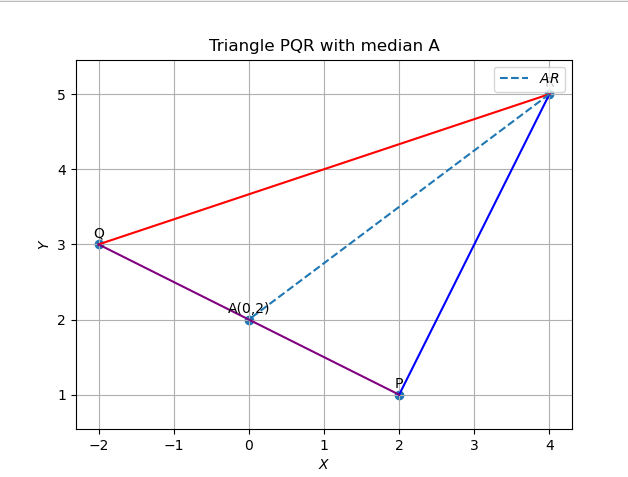
\includegraphics[width=\columnwidth]{line.png}
    \label{fig:my_label}
\end{figure}


\section*{Construction}
The dimensions of the Triangle made by using Python  are taken as below\\
\linebreak
{
\centering
	\begin{tabular}{|c|c|}
	\hline
	\textbf{vertex}&\textbf{co-ordinates}\\
	\hline
	P&(2,1)\\
	\hline
	Q&(-2,3)\\
	\hline
	R&(4,5)\\
	\hline
	A&(0,2)\\
	\hline
\end{tabular}
}
\section{\textbf{Code Link}}

\begin{lstlisting}
https://github.com/aadrshptel/Fwc_module1/tree/main/Assignments/Matrix%20assignments/Lines/codes
\end{lstlisting}
Execute the code by using the command\\
\textbf{python3 line.py}



\end{document}
